\documentclass{article}
\usepackage[T1]{fontenc}
\usepackage{lmodern}
\usepackage{graphicx}
\usepackage{amsmath,amssymb}
\usepackage[a4paper,margin=2cm]{geometry}
\usepackage[absolute,overlay]{textpos}
\setlength{\TPHorizModule}{1mm}
\setlength{\TPVertModule}{1mm}
\usepackage[indonesian]{babel}
\usepackage{hyperref}
\setlength{\emergencystretch}{2em}
% unit: Halaman 30

\begin{document}

% === Halaman 30 (llm) ===

\begin{itemize}
    \item Misalkan plainteks adalah:
    \[ P: 0101\ 0111\ 0001\ 1001\ 0110\ 0100...\ (571964\text{ dalam Hexa}) \]
    Keystream yang dibangkitkan:
    \[ K: 111101011001001000111101011... \]
    \item Enkripsi: $C = P \oplus K$
    \vspace{10mm}
    \item Dekripsi: $P = C \oplus K$
    \vspace{10mm}
\end{itemize}

\vspace{49.60mm}

% deskripsi: Ilustrasi perhitungan operasi XOR antara plainteks P dan keystream K untuk mendapatkan cipherteks C, lengkap dengan konversi hasil biner ke hexadecimal.
% bbox normalisasi: [0.1770, 0.4150, 0.6500, 0.6300]
\begin{textblock*}{99.33mm}(37.17mm,123.25mm)
\noindent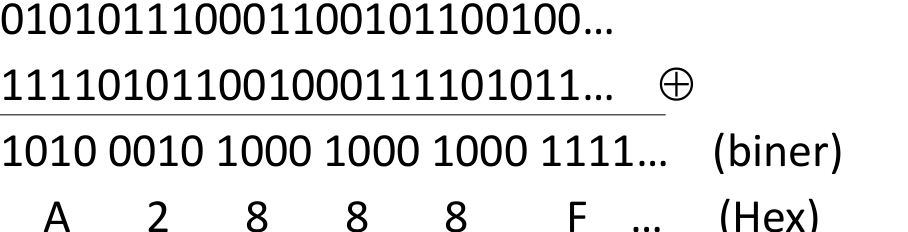
\includegraphics[width=99.33mm,height=63.86mm]{../../images/llm/page_030_img_01.png}%
\end{textblock*}

% deskripsi: Ilustrasi perhitungan operasi XOR antara cipherteks C dan keystream K untuk mengembalikan plainteks P awal dalam bentuk biner dan hexadecimal.
% bbox normalisasi: [0.1770, 0.7180, 0.7700, 0.8850]
\begin{textblock*}{124.53mm}(37.17mm,213.25mm)
\noindent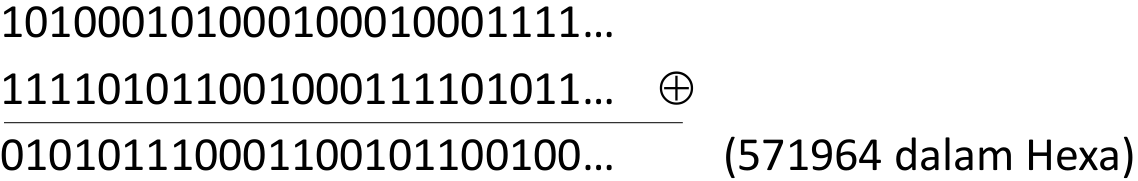
\includegraphics[width=124.53mm,height=49.60mm]{../../images/llm/page_030_img_02.png}%
\end{textblock*}

\end{document}
